\documentclass[12pt]{article}
\usepackage{amsmath, amsthm, amsfonts, amssymb}
\usepackage{graphicx} % for images

% Define theorem and lemma environments
\newtheorem{theorem}{Theorem}
\newtheorem{lemma}{Lemma}
\newtheorem{definition}{Definition}

\begin{document}

\title{Bayesian-Optimal Multi-Classification with Noisy Input Necessitates
General Input Space Representation}

\author{Aman Bhargava}

\date{\today}
\maketitle

\section{Introduction}
Here we analyze the latent representations in Bayesian filter models trained to
perform multi-class classification on some ground truth input vector 
$\mathbf x^* = [x_1^*, x_2^*]^\top$ 
based on noisy discrete-time measurement signals
$\mathbf X(t) = [X_1(t), X_2(t)]^\top$ defined as  
\begin{align}
	\label{eqn:def_noisy_input}
	X_1(t) &= x_1^* + \eta \mathcal N(0, 1) \\
	X_2(t) &= x_2^* + \eta \mathcal N(0, 1) 
\end{align}
The multi-classification task may be defined in terms of $N$ classification
boundary angles which we collectively denote as $\Theta$: 
\begin{equation}
	\label{eqn:boundaries}
	\Theta = \{\alpha_i : \alpha_i \in [-\pi, \pi], i = 1, \dots, N\}
\end{equation}
as in Figure~\ref{fig:2a}. 
\begin{figure}[h! tbp]
	\centering 
	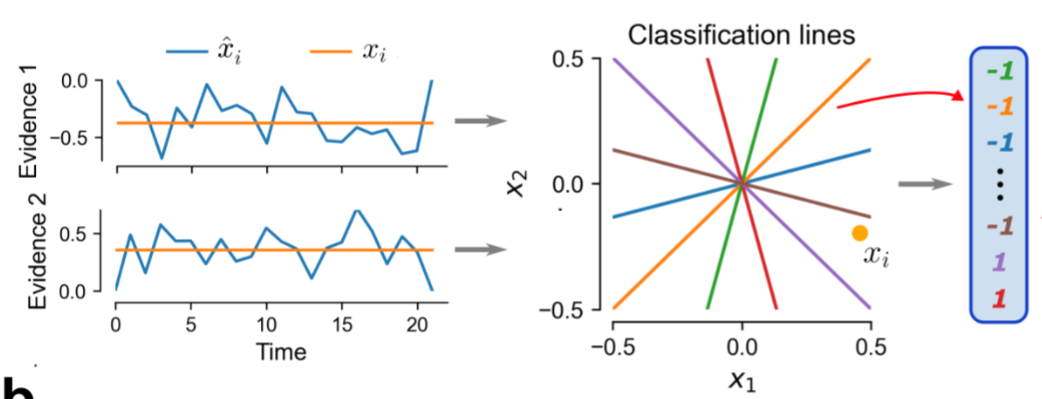
\includegraphics[width=0.9\textwidth]{media/multitask_fig2a.png}
	\caption[Multitasking RNN learns abstract representations]{\textbf{Multitasking RNN learns abstract representations. } Data generating process. The task is to simultaneously report whether the true joint evidence $(x_1,x_2)$ (yellow dot) lies above ($+1$) or below ($-1$) a number of classification lines (here 6).}
	\label{fig:2a}
\end{figure}
% The classification boundary for $\alpha_i$ is the line $x_2 = x_1 \tan \alpha_i$. 
Thus models must predict the ground truth label 
$\mathbf y^* = [y_1^* \dots y_N^*]^\top$ 
corresponding to some $\mathbf x^*$ based on the resulting noisy measurement
signals $\mathbf X(t)$ where 
\begin{equation}
	\label{eqn:def_multiclass_output}
	y_i^* = \begin{cases}
		+1 & \text{ if $x_2^* > x_1^* \tan \alpha_i$} \\
		-1 & \text{ otherwise }
	\end{cases}
\end{equation}

\paragraph{Contribution: } In this document, I demonstrate that a
Bayesian-optimal multi-classifier with noisy random input $\mathbf X(t)$ and
classification estimate output $\hat {\mathbf y}(t) \in [-1, 1]^N$ must form
latent representations $\mathbf z(t)$ that retain the 2-dimensional structural
information of the input data space $[x_1^*, x_2^*] \in \mathbb R^2$ in the
limit as $N\to \infty$ for evenly spaced $\alpha_i \in \Theta$. 
Intriguingly, without noise, we are unable to guarantee that optimal latent
representations $\mathbf z(t)$ will retain sufficient information to estimate
$\mathbf x^*$. 
While the proof is stated for 2-dimensional input, the argument should hold for
any input dimensionality. 



\subsection{Bayesian Filtering Framework}

Bayesian filters are a class of statistical models and algorithm that update a
latent state based on noisy and uncertain observation signals. 
Rooted in principles of Bayesian inference, these filters combine aggregated 
``knowledge'', represented by a latent state $\mathbf Z(t)$, with incoming
observations $\mathbf X(t)$ to continually update the latent state to
facilitate some prediction of some output $\mathbf Y(t) = f(Z(t))$. 


\begin{definition}[Bayesian Filter Operation]
	A discrete-time Bayesian filter updates latent variable $\mathbf z(t)$
	based on incoming data $\mathbf x(t)$ by applying Bayes' theorem: 
	\begin{align}
		\label{eqn:bayes_filter}
		P \big(\mathbf z(t) | \mathbf  x(t), \mathbf z(t-1)\big) &= \frac{
			P\big(\mathbf x(t) | \mathbf z(t), \mathbf z(t-1)\big) 
			P\big(\mathbf z(t) | \mathbf z(t-1)\big)
		}{
			P\big(\mathbf x(t) | \mathbf z(t-1)\big)
		} \\
		&\propto P\big(\mathbf x(t) | \mathbf z(t) \big) 
			P\big(\mathbf z(t) | \mathbf z(t-1)\big)
	\end{align}
	Bayesian filters are commonly equipped with a ``decoder'' or ``readout
	map'' $f$ which maps latent $\mathbf Z(t)$ to readout estimation
	$\hat{\mathbf Y}(t) = f(\mathbf Z(t))$.
\end{definition}

There is a deep structural similarity between RNNs and Bayesian filters, as
both models update some latent state $\mathbf z(t)$ based on incoming datum
$\mathbf x(t)$. 
Moreover, RNNs and Bayesian filters are both frequently used to predict some
value $\mathbf y(t) = f(\mathbf z(t))$ (citation: Goodfellow for RNN, Bayesian
inference textbook for filters).
We leverage the structure in the Bayesian filter formulation to prove our main
result in Section~\ref{sec:main}. 



\section{Main Results}
\label{sec:main}

Consider an optimal Bayesian filter for the multi-class classification task on 
noisy discrete time measurement signals. 



\begin{theorem}
	\label{thm:main}
	An optimal Bayesian filter trained to perform multi-class classification on
	ground truth input $\mathbf x^*$ w.r.t. decision boundaries 
	$\Theta = \{\alpha_1, \dots, \alpha_N\}$ based on noisy measurement signals
	$\mathbf X(t)$ must have latent state $\mathbf Z(t)$ that retains a
	representation of the 2-dimensional input vector $\mathbf x^*$ in the limit 
	as $N \to \infty$. 
\end{theorem}

\begin{proof}
	\begin{lemma}[Equivalence to Angle Estimation] 
		\label{lemma:angle_equiv}
		In the limit as $N\to\infty$ for uniformly distributed decision boundaries
		in $\Theta = \{\alpha_i\}_{i\in[N]}$, the multi-classification task of estimating 
		$\mathbf y^*$ (Equation~\ref{eqn:boundaries}) for a given $\mathbf x^*$
		given noisy observations $\mathbf X(t)$ is equivalent to estimating the
		angle $\theta = \angle \mathbf x^*$. 
	\end{lemma}

	\begin{lemma}[Angle Estimation Requires Magnitude Estimation]
		\label{lemma:angle_to_magnitude}
		An optimal Bayesian filter predicting the angle of some ground 
		truth input $\angle \mathbf x^*$ based on noisy observations 
		$\mathbf X(t)$ must implicitly estimate both the angle and the 
		magnitude of $\mathbf x^*$ within its latent $\mathbf Z(t)$. 
	\end{lemma}
	\begin{proof}
		Recall that the update rule latent $\mathbf Z(t)$ in the Bayesian 
		filter 
	\end{proof}

\end{proof}

% Repeat for additional theorems/lemmas if necessary

\section{Conclusion}
% Your concluding remarks.

\end{document}
